\documentclass[spanish,a4paper,14pt,oneside]{extreport}

%%%%%%%%%%%%%%%%%%%%%%%%%%%%%%%%%%%%%%%%%%%%%%%%%%%%%%%%%%%%%%%%%%%%%%%%%%%%%%%
\usepackage[dvips]{graphicx}
\usepackage[dvips]{epsfig}
\usepackage[utf8]{inputenc}
\usepackage[spanish]{babel}
\usepackage{alltt}
\usepackage{algorithm}
\usepackage{algorithmic}
\usepackage[procnumbered,ruled,algo2e]{algorithm2e}
\usepackage{multirow}
\usepackage{caption}
\usepackage{amsmath}
\usepackage{booktabs}
\usepackage[table,xcdraw]{xcolor}
\usepackage{rotating,tabularx}
\setcounter{MaxMatrixCols}{20}
\usepackage{amstext} % for \text macro
\usepackage{array}   % for \newcolumntype macro
\newcolumntype{L}{>{$}l<{$}} % math-mode version of "l" column type
\usepackage[top=2cm, bottom=2cm, left=2cm, right=2cm]{geometry}
%%%%%%%%%%%%%%%%%%%%%%%%%%%%%%%%%%%%%%%%%%%%%%%%%%%%%%%%%%%%%%%%%%%%%%%%%%%%%%%

\newcommand{\SONY}{{\sc Sony}}
\newcommand{\MICROSOFT}{{\sc Microsoft}}
\newcommand{\GCC}{\textsf{\textsc{G}CC}}
\newcommand{\INTEL}{\textsf{\textsc{I}ntel}}

%%% Traducimos el pseudocodigo
\renewcommand{\algorithmicwhile}{\textbf{mientras}}
\renewcommand{\algorithmicend}{\textbf{fin}}
\renewcommand{\algorithmicdo}{\textbf{hacer}}
\renewcommand{\algorithmicif}{\textbf{si}}
\renewcommand{\algorithmicthen}{\textbf{entonces}}
\renewcommand{\algorithmicrepeat}{\textbf{repetir}}
\renewcommand{\algorithmicuntil}{\textbf{hasta que}}
\renewcommand{\algorithmicelse}{\textbf{en otro caso}}
\renewcommand{\algorithmicfor}{\textbf{para}}

%\newcommand{\RETURN}{\textbf{retornar} }
\newcommand{\RET}{\STATE \textbf{retornar} }
\newcommand{\TO}{\textbf{hasta} }
\newcommand{\AND}{\textbf{y} }
\newcommand{\OR}{\textbf{o} }

%%%%%%%%%%%%%%%%% Creamos un entorno para listar código fuente %%%%%%%%%%%%%%%
\newenvironment{sourcecode}
{\begin{list}{}{\setlength{\leftmargin}{1em}}\item\scriptsize\bfseries}
{\end{list}}

\newenvironment{littlesourcecode}
{\begin{list}{}{\setlength{\leftmargin}{1em}}\item\tiny\bfseries}
{\end{list}}

\newenvironment{summary}
{\par\noindent\begin{center}\textbf{Abstract}\end{center}\begin{itshape}\par\noindent}
{\end{itshape}}

\newenvironment{keywords}
{\begin{list}{}{\setlength{\leftmargin}{1em}}\item[\hskip\labelsep \bfseries Keywords:]}
{\end{list}}

\newenvironment{palabrasClave}
{\begin{list}{}{\setlength{\leftmargin}{1em}}\item[\hskip\labelsep \bfseries Palabras clave:]}
{\end{list}}


%%%%%%%%%%%%%%%%%%%%%%%%%%%%%%%%%%%%%%%%%%%%%%%%%%%%%%%%%%%%%%%%%%%%%%%%%%%%%%%
% Format
%%%%%%%%%%%%%%%%%%%%%%%%%%%%%%%%%%%%%%%%%%%%%%%%%%%%%%%%%%%%%%%%%%%%%%%%%%%%%%%
%\usepackage{showframe}
%\marginparwidth 0mm
%%\topmargin -4 mm
%\topmargin -21 mm
%\headheight 10 mm
%\headsep 10 mm

%\textheight 229 mm
%\textheight 246 mm

%\oddsidemargin -5.4 mm
%\evensidemargin -5.4 mm
%\oddsidemargin 5 mm
%\evensidemargin 5 mm

%\oddsidemargin -3 mm
%\evensidemargin -3 mm

%\textwidth 17 cm
%\textwidth 15 cm
%\columnsep 10 mm

\input{amssym.def}

%%%%%%%%%%%%%%%%%%%%%%%%%%%%%%%%%%%%%%%%%%%%%%%%%%%%%%%%%%%%%%%%%%%%%%%%%%%%%%%

\begin{document}

%%%%%%%%%%%%%%%%%%%%%%%%%%%%%%%%%%%%%%%%%%%%%%%%%%%%%%%%%%%%%%%%%%%%%%%%%%%%%%%
% First Page
%%%%%%%%%%%%%%%%%%%%%%%%%%%%%%%%%%%%%%%%%%%%%%%%%%%%%%%%%%%%%%%%%%%%%%%%%%%%%%%

\pagestyle{empty}
\thispagestyle{empty}


\newcommand{\HRule}{\rule{\linewidth}{1mm}}
\setlength{\parindent}{0mm}
\setlength{\parskip}{0mm}

\vspace*{\stretch{0.5}}

\begin{center}

\includegraphics[scale=0.8]{images/logo_vertical}\\[10mm]
{\Huge Trabajo de Fin de Grado}
\end{center}

\HRule
\begin{flushright}
        {\Huge Desarrollo Dirigido por Retos} \\[2.5mm]
        {\Large \textit{Challenge-driven development}.} \\[5mm]
        {\Large Alejandro Marrero Díaz} \\[5mm]


\end{flushright}
\HRule
\vspace*{\stretch{2}}
\begin{center}
  \Large La Laguna, \today
\end{center}

\setlength{\parindent}{5mm}

%%%%%%%%%%%%%%%%%%%%%%%%%%%%%%%%%%%%%%%%%%%%%%%%%%%%%%%%%%%%%%%%%%%%%%%%%%%%%%%
% Signature page (add the official stamp)
%%%%%%%%%%%%%%%%%%%%%%%%%%%%%%%%%%%%%%%%%%%%%%%%%%%%%%%%%%%%%%%%%%%%%%%%%%%%%%%
\newpage
%\cleardoublepage
\thispagestyle{empty}

D. {\bf Eduardo Manuel Segredo González}, con N.I.F. 78.564.242-Z
profesor
Titular de Universidad
adscrito al Departamento
de Nombre del Departamento
de la Universidad de La Laguna, como tutor

\bigskip
D. {\bf Carlos Segura González}, con N.I.F. 78.704.244-S
profesor
Titular de Universidad
adscrito al Departamento
de Nombre del Departamento
de la Universidad de La Laguna, como cotutor

\bigskip
\bigskip
{\bf C E R T I F I C A N}

\bigskip
\bigskip
\bigskip
Que la presente memoria titulada:

\bigskip
``{\it Desarrollo Dirigido por Retos.}''

\bigskip
\bigskip
\bigskip

\noindent ha sido realizada bajo su dirección por D. {\bf Alejandro Marrero Díaz},
con N.I.F. 78.649.404-F.

\bigskip
\bigskip

Y para que así conste, en cumplimiento de la legislación vigente y a los efectos
oportunos firman la presente en La Laguna a \today

%\cleardoublepage
\newpage
%%%%%%%%%%%%%%%%%%%%%%%%%%%%%%%%%%%%%%%%%%%%%%%%%%%%%%%%%%%%%%%%%%%%%%%%%%%%%%%
\thispagestyle{empty}

{ \flushright

\begin{LARGE}
Agradecimientos
\end{LARGE}

\hspace{3mm}

\begin{large}


\hspace{3mm}
A mi familia y amigos que

\hspace{3mm}
me han apoyado incondicionalmente estos 4 años.

\bigskip

\hspace{3mm}
Agradecer también a los directores de este proyecto,

\hspace{3mm}
Eduardo Segredo y Carlos Segura,

\hspace{3mm}
por la ayuda en el desarrollo de este proyecto

\hspace{3mm}
y por adentrarme en el mundo de la investigación.

\end{large}

}

%%%%%%%%%%%%%%%%%%%%%%%%%%%%%%%%%%%%%%%%%%%%%%%%%%%%%%%%%%%%%%%%%%%%%%%%%%%%%%%%%
\newpage

\begin{huge}
Licencia
\end{huge}
\begin{center}

\includegraphics[scale=1.5]{images/by-nc-sa_88x31}\\[10mm]
{\Large \copyright~Esta obra está bajo una licencia de Creative Commons Reconocimiento-NoComercial-CompartirIgual 4.0 Internacional.
}
\end{center}



%%%%%%%%%%%%%%%%%%%%%%%%%%%%%%%%%%%%%%%%%%%%%%%%%%%%%%%%%%%%%%%%%%%%%%%%%%%%%%%
\newpage  %\cleardoublepage
\begin{abstract}
{\em

Con este Trabajo de Fin de Grado se ha buscado adentrar al alumno en el mundo de la investigación, y concretamente, en el campo de las meta-heurísticas. Para ello, se han implementado diversas técnicas algorítmicas, incluyendo algunas técnicas pertenecientes a la familia de los algoritmos evolutivos, así como otras técnicas meta-heurísticas poblacionales de trayectoria.

\bigskip

Para evaluar el rendimiento de los algoritmos implementados, 
se ha participado en una competición de optimización global continua denominada 
Generalization-based Contest in Global Optimization (GenOpt).

\bigskip

En concreto, se han implementado los algoritmos Opposition-Based-Learning Competitive-Particle Swarm Optimization, Covariance Matrix Adaptation Evolutionary Strategy y Simulated Annealing los cuales se han aplicado a los problemas propuestos por la competición GenOpt. La elección de estos algoritmos se basa en la demostración de su buen desempeño en problemas de optimización global continua. Además de los tres algoritmos mencionados, se ha desarrollado el conjunto de métricas, especificadas en el manifiesto de la competición, necesarias para evaluar el rendimiento de los algoritmos desarrollados.

}

\begin{palabrasClave}
Optimización Global Continua, Meta-heurísticas, Computación Evolutiva, Ajuste De Parámetros.
\end{palabrasClave}

\end{abstract}
%%%%%%%%%%%%%%%%%%%%%%%%%%%%%%%%%%%%%%%%%%%%%%%%%%%%%%%%%%%%%%%%%%%%%%%%%%%%%%%

%%%%%%%%%%%%%%%%%%%%%%%%%%%%%%%%%%%%%%%%%%%%%%%%%%%%%%%%%%%%%%%%%%%%%%%%%%%%%%%
\newpage  %\cleardoublepage
\begin{summary}
{\em

The main goal of this degree thesis is to introduce the student to the research field through the application of several meta-heuristic approaches to global continuous optimization problems. For doing that, we have developed several algorithmic techniques, including some methods belonging to the family of evolutionary algorithms, as well as other population and trajectory-based meta-heuristics.

In order to assess the performance of the implemented schemes, we have participated in a competition on global continuous optimization referred to as Generalization-based Contest in Global Optimization (GENOPT). The main aim of this competition is diversify the number of approaches solving the proposed problems.

In particular, we have implemented the algorithms Opposition-based Learning Competitive Particle Swarm Optimization, Covariance Matrix Adaptation Evolution Strategy and Simulated Annealing, which have been applied to solve the problems proposed by the GENOPT. The aforementioned algorithms were chosen because they have shown to provide better performance in comparison to other alternatives when dealing with global continuous optimization problems. In addition to the above, we have also implemented a set of metrics proposed by the competition organization with the aim of measuring the performance of our algorithmic proposals.

}

\begin{keywords}
Global Continuos Optimization,, Meta-heuristics, Evolutionary Computation, Parameter Setting.
\end{keywords}

\end{summary}
%%%%%%%%%%%%%%%%%%%%%%%%%%%%%%%%%%%%%%%%%%%%%%%%%%%%%%%%%%%%%%%%%%%%%%%%%%%%%%%

%%%%%%%%%%%%%%%%%%%%%%%%%%%%%%%%%%%%%%%%%%%%%%%%%%%%%%%%%%%%%%%%%%%%%%%%%%%%%%%
\newpage{\pagestyle{empty}}
\thispagestyle{empty}

%%%%%%%%%%%%%%%%%%%%%%%%%%%%%%%%%%%%%%%%%%%%%%%%%%%%%%%%%%%%%%%%%%%%%%%%%%%%%%%


\pagestyle{myheadings} %my head defined by markboth or markright
% No funciona bien \markboth sin "twoside" en \documentclass, pero al
% ponerlo se dan un montón de errores de underfull \vbox, con lo que no se
% ha puesto.
\markboth{Alejandro Marrero Díaz}{Desarrollo Dirigido por Retos}

%%%%%%%%%%%%%%%%%%%%%%%%%%%%%%%%%%%%%%%%%%%%%%%%%%%%%%%%%%%%%%%%%%%%%%%%%%%%%%%
%Numeracion en romanos
\renewcommand{\thepage}{\roman{page}}
\setcounter{page}{1}

%%%%%%%%%%%%%%%%%%%%%%%%%%%%%%%%%%%%%%%%%%%%%%%%%%%%%%%%%%%%%%%%%%%%%%%%%%%%%%%

\tableofcontents

%%%%%%%%%%%%%%%%%%%%%%%%%%%%%%%%%%%%%%%%%%%%%%%%%%%%%%%%%%%%%%%%%%%%%%%%%%%%%%%
\newpage{\pagestyle{empty}}

\listoffigures

%%%%%%%%%%%%%%%%%%%%%%%%%%%%%%%%%%%%%%%%%%%%%%%%%%%%%%%%%%%%%%%%%%%%%%%%%%%%%%%
\newpage{\pagestyle{empty}}

\listoftables

%%%%%%%%%%%%%%%%%%%%%%%%%%%%%%%%%%%%%%%%%%%%%%%%%%%%%%%%%%%%%%%%%%%%%%%%%%%%%%%
\newpage{\pagestyle{empty}}

%%%%%%%%%%%%%%%%%%%%%%%%%%%%%%%%%%%%%%%%%%%%%%%%%%%%%%%%%%%%%%%%%%%%%%%%%%%%%%%
%Numeracion a partir del capitulo I
\renewcommand{\thepage}{\arabic{page}}
\setcounter{page}{1}


\chapter{Introducción}
\label{chapter:intro}

%%%%%%%%%%%%%%%%%%%%%%%%%%%%%%%%%%%%%%%%%%%%%%%%%%%%%%%%%%%%%%%%%%%%%%%%%%%%%
% Chapter 1: Introducción 
%%%%%%%%%%%%%%%%%%%%%%%%%%%%%%%%%%%%%%%%%%%%%%%%%%%%%%%%%%%%%%%%%%%%%%%%%%%%%%%

%---------------------------------------------------------------------------------
\section{Descripción del Trabajo de Fin de Grado}
\label{sec:DESCRIPTION}

En este Trabajo de Fin de Grado, se propone el diseño y análisis de diversas técnicas algorítmicas para la resolución de problemas definidos en el ámbito de un concurso/competición de optimización.
	En la actualidad,  muchos de los problemas del mundo real se pueden formular como problemas de optimización con variables de decisión cuyos valores varían en un dominio continuo. Es por eso que podemos encontrar una gran cantidad de competiciones en esta materia que fomentan la cooperación y la investigación en el campo de la computación. Aunque son muchas las técnicas que pueden ser empleadas para resolver este tipo de problemas, se ha probado que la utilización de metaheurísticas y otras técnicas de computación evolutiva (EC, del inglés, Evolutionary Computation), como la familia de algoritmos evolutivos, presentan numerosas y exclusivas ventajas como:
Robustez y fiabilidad.
Capacidad de búsqueda global.
Abstracción del dominio del problema a resolver.

Además de las ventajas anteriormente mencionadas, las técnicas de computación evolutiva nos proporcionan otras características como pueden ser la facilidad con la que pueden ser implementadas y la posibilidad de paralelizarlas de un modo relativamente sencillo.
	Por lo tanto, el principal objetivo del presente Trabajo de Fin de Grado es el diseño, desarrollo y análisis de la parametrización de diversos algoritmos evolutivos y otras técnicas metaheurísticas en el ámbito de una competición de optimización continua. 
%---------------------------------------------------------------------------------
\section{Antecedentes y Estado Actual del Tema}
\label{sec:SUBJECT}

Como se ha indicado en el apartado anterior, actualmente existen una gran cantidad de competiciones de optimización organizadas en diferentes congresos como son:
\begin{itemize}
  \item Congress on Evolutionary Computation - CEC 2017.
  \item Genetic and Evolutionary Computation Conference - GECCO 2017.
  \item Global Trajectory Optimisation Competition - GTOC.
  \item International Conference on Evolutionary Multi-Criterion Optimization - EMO 2017.
  \item Generalization-based Contest in Global Optimization - GENOPT.
\end{itemize}

En concreto, este Trabajo de Fin de Grado se basará en la resolución de los problemas de optimización global continua descritos en GENOPT. En esta competición se propone la minimización de 18 funciones con 10 o 30 variables de decisión, las cuales se dividen en tres familias diferentes: funciones GKLS, funciones de benchmark clásicas transformadas, y funciones compuestas.
Las primera familia de funciones se obtiene mediante un generador GKLS que permite obtener tres clases de funciones con los valores mínimos locales y globales conocidos para realizar una optimización global multidimensional de tipo “box-constrained”.
La segunda familia de funciones se basan en problemas de benchmark de optimización continua clásicos, de dificultad variable.
\newline
Por último, la última familia se obtiene realizando una composición de funciones pertenecientes a la segunda familia, generando seis tipos diferentes de problemas.	
Se puede obtener más información al respecto en el Manifesto GENOPT.
Por otra parte, como se comentó en el apartado de introducción, se estudiarán diversos algoritmos evolutivos y otro tipo de metaheurísticas para la resolución de los problemas planteados. En este caso, cabe destacar los algoritmos Particle Swarm Optimization (PSO), Differential Evolution (DE) y Covariance Matrix Adaptation Evolution Strategy (CMA-ES), entre otros. Otro posible objeto de estudio serán diversas técnicas de inicialización de algoritmos, principalmente, la familia de técnicas Opposition-Based Learning (OBL).


%%%%%%%%%%%%%%%%%%%%%%%%%%%%%%%%%%%%%%%%%%%%%%%%%%%%%%%%%%%%%%%%%%%%%%%%%%%%%%%

\chapter{Conceptos previos}
\label{chapter:dos}
%%%%%%%%%%%%%%%%%%%%%%%%%%%%%%%%%%%%%%%%%%%%%%%%%%%%%%%%%%%%%%%%%%%%%%%%%%%%%%%
% Chapter 2: Título del capítulo 2
%%%%%%%%%%%%%%%%%%%%%%%%%%%%%%%%%%%%%%%%%%%%%%%%%%%%%%%%%%%%%%%%%%%%%%%%%%%%%%%

%++++++++++++++++++++++++++++++++++++++++++++++++++++++++++++++++++++++++++++++

%++++++++++++++++++++++++++++++++++++++++++++++++++++++++++++++++++++++++++++++
\section{Optimización Global}
\label{sec:OPT}
%%%%%%%%%%%%%%%%%%%%%%%%%%%%%%%%%%%%%%%%%%%%%%%%%%%%%%%%%%%%%%%%%%%%%%%%%%%%%%


La Optimización Global trata de optimizar una función dentro de un intervalo especificado y teniendo en cuenta diversos criterios y/o restricciones. Por lo general, el objetivo de la optimización global es la de encontrar el óptimo (mínimo o máximo) u óptimos globales de la función $f$ a optimizar, tratando de evitar posibles óptimos locales. 
La optimización global se basa en encontrar aquel valor mínimo o máximo global dentro del espacio de búsqueda de la función \textbf{\textit{f}} a optimizar. La elección de la técnica empleada para encontrar el óptimo global resulta resulta de gran importancia dado que la función \textbf{\textit{f}} puede tener muchos óptimos locales que pueden llevar al algoritmo a \textbf{converger prematuramente}, sin que luego pueda escapar de estos óptimo locales. \\
De manera formal, el objetivo de la optimización global, considerando un problema de minimización, es encontrar un vector $X* \in \Omega$ tal que $f(X*) \leq f(X)$ para todo $X \in \Omega$ \cite{Segredo2017}.
En este caso particular, tratamos la optimización de tipo \textbf{\textit{box-constrained}}, donde \textbf{el espacio de búsqueda} $\Omega$ está definido por un límite inferior ($a_{i}$) y superior ($b_{i}$) para cada una de las variables de decisión de la función, es decir: $\Omega = \prod^{D}_{i=1}[a_{i}, b{i}]$, siendo D el número de variables de decisión del problema a optimizar \cite{Segredo2017}.


%%%%%%%%%%%%%%%%%%%%%%%%%%%%%%%%%%%%%%%%%%%%%%%%%%%%%%%%%%%%%%%%%%%%%%%%%%%%%%
\section{Técnicas Meta-heurísticas}
\label{sec:META}
%%%%%%%%%%%%%%%%%%%%%%%%%%%%%%%%%%%%%%%%%%%%%%%%%%%%%%%%%%%%%%%%%%%%%%%%%%%%%%

Las meta-heurísticas son un sub-conjunto de métodos de optimización que se encuentran incluidas dentro del conjunto de métodos heurísticos que a su vez forman parte de los métodos aproximados.

\begin{figure}
  \centering
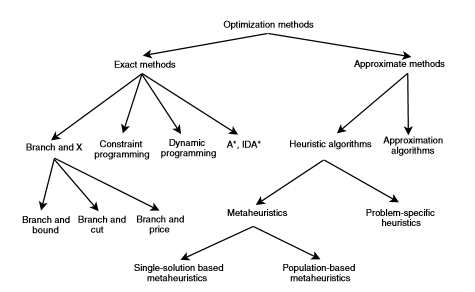
\includegraphics[scale=1.0]{images/meta}\\[10mm]
  \caption{Métodos de optimización.}
\end{figure}

A diferencia de los métodos de optimización exactos, las meta-heurísticas nos permiten obtener soluciones factibles a problemas complejos en un tiempo aceptable, aunque no nos garantizan obtener la solución óptima global \cite{metaheuristics}. En los últimos años estás técnicas algorítmicas han ganado una gran popularidad dado que han demostrado su efectividad y eficiencia en muchos campos y con una gran cantidad de problemas distintos.

En cuanto a las distintas meta-heurísticas que podemos encontrar hoy en día, podemos diferenciar las siguientes categorías \cite{metaheuristics}:

\begin{itemize}
    \item \textbf{Búsquedas Locales}: Greedy Randomized Adaptive Search Procedure (GRASP) \cite{GRASP}, Variable neighborhood search (VNS) \cite{vns}.
    \item \textbf{Heurísticas Voraces}: Simulated Annealing (SA) \cite{SA}.
    \item \textbf{Algoritmos Evolutivas}: Covariance Matrix Adaptation Evolutionary Strategy (CMA-ES) \cite{CMA}, Differential Evolution (DE) \cite{DE1, DE2, DE3}, Coevolutionary algorithms (CEA) \cite{COE1, COE2, COE3}.
\end{itemize}


Esta gran variedad de técnicas se debe principalmente al gran abanico de criterios que podemos definir a la hora de diseñar una meta-heurística. Generalmente, las meta-heurísticas, y en especial, los algoritmos evolutivos, buscan un balance entre las propiedades de intensificación y diversificación. El concepto de intensificación significa aprovechar una solución prometedora  obtenida y tratar de explotar la región del espacio de búsqueda cercana a la misma en busca de posibles mejores soluciones, mientras, mientras que la diversificación se caracteriza por priorizar la búsqueda por las diferentes áreas no exploradas del espacio de búsqueda. Sin embargo, algunas técnicas como la búsqueda local, se centran principalmente en intensificar. Otra clasificación agrupa las diferentes meta-heurísticas en las siguientes clases:

\begin{itemize}
    \item \textbf{Métodos inspirados en la naturaleza}: es común inspirarse en el comportamiento de animales o bien de procesos físicos para diseñar un método meta-heurístico que emule ese comportamiento. Por ejemplo: Ant Bee Colonies \cite{Mann2017} y Simulated Annealing \cite{SA}.
    \item \textbf{Determinísticos o Estocásticos}: podemos optar por tomar decisiones deterministas o emplear reglas aleatorias durante la búsqueda de nuevas soluciones. Por ejemplo: Simulated Annealing \cite{SA1}.
    \item \textbf{Métodos basados en poblaciones o basados en una única solución}: Por un lado nos podemos basar en un conjunto de soluciones factibles que combinaremos entre ellas aplicando diversos operadores para obtener un  nuevo conjunto de soluciones potencialmente mejores. O bien, podemos optar por utilizar una única solución al problema que transformaremos en cada iteración del algoritmo.
    \item \textbf{Iterativos o voraces}: en este aspecto podemos contemplar comenzar con un conjunto de soluciones al problema e ir transformando dichas soluciones en cada iteración del algoritmo para obtener nuevas soluciones. Al contrario, en una estrategia voraz (Greedy) comenzamos sin una solución factible al problema y en cada iteración incluiremos una variable de decisión hasta obtener la solución completa.
\end{itemize}

\subsection{Representación}

En las técnicas algorítmicas en general nos podemos encontrar con diversas maneras de representar la solución $S$ al problema y en las meta-heurísticas estás son las más comunes \cite{metaheuristics}:

\bigskip

\begin{itemize}
    \item \textbf{Cadena binaria}: utilizada en problemas de decisiones.
    \begin{figure}[!ht]
    \centering
    
\includegraphics[scale=1.2]{images/binaria}
    \caption{Ejemplo de representación en cadena binaria.}
    \end{figure} 
    \item \textbf{Vector de valores naturales}: problemas de optimización combinatoria.
    \begin{figure}[!ht]
    \centering
    
\includegraphics[scale=1.2]{images/natural}
    \caption{Ejemplo de representación en vector de números naturales.}
    \end{figure}
    \item \textbf{Vector de números reales}: utilizada en problemas de optimización continua.
    \begin{figure}[!ht]
    \centering
    
\includegraphics[scale=1.2]{images/reales}
    \caption{Ejemplo de representación en vector de números reales.}
    \end{figure}
    \item \textbf{Secuencia}: empleada en problemas de rutas y de planificación de tareas.
    \begin{figure}[!ht]
    \centering
    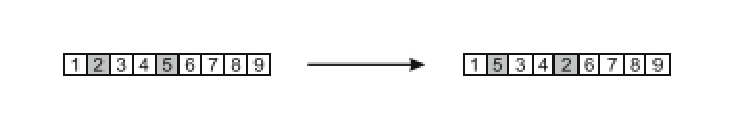
\includegraphics[scale=1.2]{images/secuencia}
    \caption{Ejemplo de representación en secuencia.}
    \end{figure}
\end{itemize}

Dadas las características del concurso seleccionado para este Trabajo de Fin de Grado, la representación empleada fue \textbf{vector de valores reales} dado que cada elemento del vector denota un valor dentro del dominio de la función para cada una de las \textbf{\textit{d variables}} que posee.

\subsection{Condición de Parada}
Generalmente, las técnicas meta-heurísticas finalizan su ejecución según un criterio de finalización o \textbf{condición de parada}. Las más comunes son: 

\bigskip

\begin{itemize}
    \item \textbf{Iteraciones}: el algoritmo se detiene al alcanzar un determinado número de generaciones de individuos producidas.
    \item \textbf{Evaluaciones}: cuando el número de evaluaciones de la función objetivo a optimizar realizadas por el algoritmo llega a un valor prefijado, el algoritmo finaliza su ejecución.
    \item \textbf{Factor de error}: al alcanzar un factor de error lo suficientemente bajo como para considerar la solución óptima, el algoritmo detiene su ejecución.
\end{itemize}

En nuestro trabajo, el criterio de parada utilizado por todos los algoritmos desarrollados es \textbf{$10^{6}$ evaluaciones}, criterio prefijado por la organización del concurso GenOpt. 


%%%%%%%%%%%%%%%%%%%%%%%%%%%%%%%%%%%%%%%%%%%%%%%%%%%%%%%%%%%%%%%%%%%%%%%%%%%%%%%
\newpage{\pagestyle{empty}}
\thispagestyle{empty}

\chapter{Técnicas Algorítmicas Desarrolladas}
\label{chapter:tres}

%%%%%%%%%%%%%%%%%%%%%%%%%%%%%%%%%%%%%%%%%%%%%%%%%%%%%%%%%%%%%%%%%%%%%%%%%%%%%%%
% Chapter 3: Título del capítulo 3
%%%%%%%%%%%%%%%%%%%%%%%%%%%%%%%%%%%%%%%%%%%%%%%%%%%%%%%%%%%%%%%%%%%%%%%%%%%%%%%

%++++++++++++++++++++++++++++++++++++++++++++++++++++++++++++++++++++++++++++++

\section{Opposition-based Learning (OBL)}
\label{sec:OBL}
%%%%%%%%%%%%%%%%%%%%%%%%%%%%%%%%%%%%%%%%%%%%%%%%%%%%%%%%%%%%%%%%%%%%%%%%%%%%%%

Opposition-based Learning (OBL)\cite{obl, obl2, OPSO, OPSO2, OPSO3} es un concepto en computación que ha demostrado gran efectividad a la hora de mejorar diversas técnicas de optimización. Cuando evaluamos una solución X candidata para un problema dado, simultáneamente  
 calcularemos la solución opuesta $\overline{X}$, consiguiendo así una mayor exploración del espacio de búsqueda $\Omega$ en busca del óptimo global \cite{obl}. Asimismo, podemos encontrar diversas variantes a la estrategia tradicional de OBL como pueden ser: Quasi-opposition-based Learning (QOBL), Quasi-reflected Opposition-based Learning (QROBL).

Sea $x \in \Re $  un número real definido dentro de un cierto intervalo: $x \in [a,b]$. El número opuesto de x denotado como $\overline{x}$ se define de la siguiente forma\cite{obl}: \\
 \begin{equation}
     \overline{x} = a + b - x  \\
 \end{equation}

Análogamente, para el caso de optimizar una función n-dimensional la solución opuesta se calcularía de la siguiente forma: \\

 Sea $ P(x_{1}, x_{2},...,x_{n}) $ un punto dentro de un sistema de coordenadas n-dimensional con $ x_{1},...,x_{n} \in \Re$ y además $ x_{i} \in [a_{i}, b{i}]$. \cite{obl} El opuesto del punto P se define como las coordenadas $\overline{x_{1}},...\overline{x_{n}}$ donde:\\
\begin{equation}
    \overline{x_{i}} = a_{i} + b_{i} - x_{i} \quad i = 1,...,n \\
\end{equation}

En nuestro desarrollo hemos empleado este concepto en varios procesos, como puede ser el proceso de inicialización de los individuos que formarán parte de la primera población o bien, tras cada iteración del algoritmo como medida de diversificación. 

%%%%%%%%%%%%%%%%%%%%%%%%%%%%%%%%%%%%%%%%%%%%%%%%%%%%%%%%%%%%%%%%%%%%%%%%%%%%%%%
\section{Búsqueda Global}\label{sec:BG}

En ciencias de la computación, una búsqueda global (Global Search) es un método heurístico para resolver problemas complejos de optimización \cite{GlobalSearch, GlobalSearch2, GlobalSearch3}. %Una búsqueda global puede formularse como encontrar una solución óptima dentro de un conjunto de soluciones factibles: \\
%\begin{equation}
 %   X' \in \Omega \quad \land \quad f(x')\leq f(x)
%\end{equation}
%
El funcionamiento básico de una búsqueda global se basa en que el algoritmo se mueve dentro del espacio de búsqueda explorando todas las soluciones factibles y aplicando cambios a cada una de ellas hasta encontrar una solución óptima. 

Para nuestro trabajo, hemos diseñado una búsqueda global que \textbf{se aplicará como último paso en cada iteración de los algoritmos} que hemos desarrollado con el objetivo de obtener una mayor diversificación y escapar de los posibles óptimos locales. En primer lugar, el procedimiento calculará el individuo centroide de la población. El centroide de un conjunto n-dimensional de $k$ elementos se define como:
\begin{equation}\label{centroide}
    C = \frac{x_{1} + x_{2} + ... + x_{k}}{k}
\end{equation}

Para nuestro caso particular, debemos tener en cuenta que cada uno de nuestros elementos $x_{i}$ representan una solución factible a nuestro problema con $d$ variables cada uno. Es por ello que, el individuo centroide se calculará de la siguiente manera: 

\begin{algorithm}[!ht]
  \caption{Cálculo del centroide(\mbox{})}
  \label{pseu:centroide}
  \begin{algorithmic}[1]
    \FOR{$i \leftarrow 0 $ hasta $D$}
      \STATE $Suma = 0$;
      \FOR{$j \leftarrow 0$ hasta $\left | S \right |$}
        \STATE $Suma = Suma + S[i][j];$
      \ENDFOR
      \STATE Centroide[i] = $\frac{Suma}{\left | S \right |}$;
    \ENDFOR    
    \RETURN Centroide
  \end{algorithmic}
\end{algorithm}
Seguidamente, pasaremos a explorar la población de individuos aplicando pequeñas modificaciones a cada uno de ellos para obtener nuevos individuos \textit{hijos}. Si estos individuos mejoran a sus ancestros serán incluidos dentro del conjunto de soluciones S y continuaremos aplicando modificaciones a su ancestro hasta que no se produzca mejora en su descendencia. En otro caso, serán descartados.
Finalmente, devolveremos una nueva población con los $|S|$ mejores individuos encontrados entre padres e hijos. \\
A continuación, podemos ver el pseudocódigo de nuestra aproximación de búsqueda global empleada en nuestros desarrollos: 


\begin{algorithm}[!ht]
  \caption{Búsqueda global(\mbox{})}
  \label{pseu:bg}
  \begin{algorithmic}[1]
    \STATE NumIndividuos = $\left | S \right |$;
    \STATE OrdenarPoblacion(S);
    \STATE MarcarNoExplorados(S);
    \STATE Centroide = CalcularCentroide();
    \STATE NumeroMejora = 0;
    \STATE NumeroExplorado = 0;
    \WHILE{$NumeroMejora > 0 $ y $NumeroExplorado < \left | S \right |$}
      \STATE k = 0;
      \WHILE{$S[k] = explorado $ y $NumeroExplorado < \left | S \right |$}
        \STATE k = rand(0, $\left | S \right |$); Buscamos un individuo $k$ no explorado
      \ENDWHILE
      \STATE S[k] = explorado;
      \STATE NumeroExplorado = NumeroExplorado + 1;
      \STATE Mejora = true;
      \WHILE{$Mejora = true$}
        \WHILE{$|a_{1}| + |a_{2}| + |a_{3}| \neq 1$}
          \STATE GenerarRand(a1, a2, a3); Obtenemos tres valores generados aleatoriamente de manera uniforme en el rango [0, 1] para realizar la modificación del individuo
        \ENDWHILE
        \WHILE{$ r_{1} < k$}
          \STATE $ r_{1}$ = rand(0, $\left | S \right |$); Buscamos un individuo $r_{1}$ aleatoriamente para usar sus variables en la generación del nuevo individuo
        \ENDWHILE
        \STATE NuevoInd = ModificarIndividuo(k, a1, a2, a3, Centroide, $r_{1}$);
        \IF{$NuevoInd < S[k]$}
          \STATE $Mejora = true;$
          \STATE $S = S \cap NuevoInd$;
          \STATE NumeroMejora = NumeroMejora + 1;
          \ELSE
            \STATE Mejora = false;
        \ENDIF
      \ENDWHILE
    \ENDWHILE
    \STATE OrdenarPoblacion(S); 
    \STATE S = ObtenerMejores(0, NumIndividuos, S);
    \RETURN $\left | S \right |$ mejores individuos encontrados
  \end{algorithmic}
\end{algorithm}




\section{OBL Competitive Particle Swarm Optimization (OBL-CPSO)}
\label{sec:OBL-CPSO}
%%%%%%%%%%%%%%%%%%%%%%%%%%%%%%%%%%%%%%%%%%%%%%%%%%%%%%%%%%%%%%%%%%%%%%%%%%%%%%

\subsection{Particle Swarm Optimization}
Particle Swarm Optimization (PSO) \cite{metabook, comparison, PSO_KA, GPSO} es una estrategia de optimización que ha demostrado ser muy eficiente en problemas de optimización global continua. Se basa en simular el conjunto de soluciones candidatas a un problema dado como un enjambre de partículas que se mueven dentro de un espacio de búsqueda definido. Dado que las partículas se mueven, estas poseen una posición \textit{x} y una velocidad \overrightarrow{v} en cada instante \textit{t} de ejecución del algoritmo. La posición \textit{x} representa los valores que toman las diferentes variables dentro de una solución y, la velocidad \overrightarrow{v}, determinará la dirección y la rapidez con la que la partícula se desplazará por el espacio de búsqueda, es decir, el factor de modificación para cada una de las variables de decisión. A parte de estas características, cada partícula tiene la capacidad de recordar su mejor posición alcanzada durante la ejecución del algoritmo, y para cada partícula $p_{i}$ la denotaremos como $pb_{i}$\cite{metabook}. Esto nos permite evaluar si el movimiento de una partícula mejora la solución actual o por el contrario es mejor permanecer en la posición actual. \\

Por otra parte, en el algoritmo PSO también se tiene en cuenta una partícula denominada \textit{global best $(gb)$} en la que se almacena la mejor posición histórica alcanzada por una partícula dentro del enjambre. Estas dos posiciones $pb_{i}$ y \textit{gb} son usadas en cada iteración del algoritmo para atraer el movimiento de las partículas hacia esas posiciones, consiguiendo así que el algoritmo PSO converga rápidamente hacia las soluciones óptimas. \\
A continuación, se muestra el esquema básico del algoritmo PSO: 
\begin{algorithm}[!ht]
  \caption{Particle Swarm Optimization(\mbox{})}
  \label{pseu:pso}
  \begin{algorithmic}[1]
    \WHILE{Condición de parada no satisfecha}
      \FORALL{$p_{i}$ en S}
        \STATE Evaluar $ p_{i} $;
        \STATE Actualizar mejor posición $pb_{i}$;
        \STATE Actualizar mejor global $gb$;
      \ENDFOR
      \FORALL{$p_{i}$ en S}
       \FORALL{$d_{i}$ en D}
       \STATE $ v_{i,d} = v_{i,d} + C_{1} * Rnd(0,1) * [pb_{i,d} - x_{i,d}] + C_{2} + Rnd(0,1) * [gb_{d} - x_{i,d}] $;\\ Rnd(0,1) devuelve un número generado aleatoriamente en el rango [0, 1]
            $ x_{i,d} = x_{i,d} + v_{i,d}$; \\
       \ENDFOR
      \ENDFOR
    \ENDWHILE
    \RETURN Mejor solución obtenida
  \end{algorithmic}
\end{algorithm}

\subsection{OBL-CPSO}
En esta ocasión, el algoritmo Opposition-based Learning Competitive Particle Swarm Optimization (OBL-CPSO) \cite{oblcpso} desarrollado incluye dos modificaciones sobre el esquema básico del algoritmo PSO como son Opposition-based Learning, detallado en el apartado \ref{sec:OBL}, y un procedimiento de competición entre las partículas que conforman el enjambre. \\

El procedimiento de competición se basa en escoger tres partículas dentro del enjambre aleatoriamente, hacerlas competir entre ellas, mediante su valor de función objetivo, obteniendo un partícula ganadora, otra perdedora y una partícula neutra para, posteriormente, eliminarlas del enjambre. Para un enjambre de tamaño N, en cada iteración del algoritmo se realizarán N/3 competiciones \cite{oblcpso}. Tras cada competición, la partícula ganadora pasará directamente a la siguiente iteración del algoritmo y la partícula perdedora pasará también a la siguiente iteración tras aprender de la partícula ganadora, es decir, la partícula ganadora atrae a la partícula perdedora hacia su posición. La partícula neutral será la escogida para utilizarla en la estrategia de OBL y seguidamente pasar a la siguiente iteración, tratando, de este modo, de mejorar la capacidad de exploración del algoritmo \cite{oblcpso}. \\

La partícula perdedora y la partícula neutral van a modificar su posición y su velocidad siguiendo las siguientes ecuaciones:

\begin{equation} \label{eq:7}
    V^{k}_{ld}(t+1) = R^{k}_{1d}(t) * V^{k}_{ld}(t) + R^{k}_{2d}(t) * (X^{k}_{wd}(t) - X^{k}_{ld}(t)) + \varphi * R^{k}_{3d}(t) * (\overline{X}^{k}_{ld}(t+1)) 
\end{equation}

\begin{equation} \label{eq:8}
     X^{k}_{ld}(t+1) = X^{k}_{ld}(t) + V^{k}_{ld}(t+1)
\end{equation}

\begin{equation} \label{eq:9}
     X^{k}_{nd}(t+1) = ub_{d} + lb_{d} - X^{k}_{nd}(t) + R^{k}_{4d}(t) * X^{k}_{nd}(t)
\end{equation}

Donde $X^{k}_{wd}(t)$, $ X^{k}_{ld}(t)$ y $ X^{k}_{nd}(t)$ son las posiciones d-ésimas de las partículas ganadora (winner), perdedora (looser) y neutral en la k-ésima ronda de competición dentro de la iteración t. $V^{k}_{ld}$ es la velocidad de la partícula perdedora en la dimensión d-ésima en la k-ésima ronda de competición de la iteración t \cite{oblcpso}. Y por último, $R^{k}_{1d}$, $R^{k}_{2d}(t)$, $R^{k}_{3d}(t)$ y $R^{k}_{4d}(t)$ son valores escogidos aleatoriamente dentro del intervalo [0,1], $\varphi$ es un parámetro fijado manualmente, $\overline{X}^{k}_{ld}(t)$ representa el valor medio de las posiciones de las partículas dentro del enjambre y, $ub_{d}$ y $lb_{d}$ son las cotas superiores e inferiores del espacio de búsqueda en la dimensión d-ésima \cite{oblcpso}. \\
El pseudocódigo del algoritmo OBL-CPSO se muestra en la siguiente figura: 
\begin{algorithm}[]
  \caption{OBL Competitive Particle Swarm Optimization(\mbox{})}
  \label{pseu:oblcpso}
  \begin{algorithmic}[1]
    \STATE Inicializar();
    \WHILE{Condición de para no satisfecha}
      \FORALL{$ k=1: N/3 $}
        \STATE $ r_{1} = S(k)$;
        \STATE $ r_{2} = S(k + N/3)$;
        \STATE $ r_{3} = S(k + 2N/3)$;
        \STATE $(w, n, l) = competir(r_{1}, r_{2}, r_{3})$;
        \STATE Actualizar $ X^{k}_{ld}(t)$; (Ec. \ref{eq:7} y Ec. \ref{eq:8})
        \STATE Actualizar $ X^{k}_{nd}(t)$; (Ec. \ref{eq:9})
        \STATE Actualizar los valores de fitness para N y L;
      \ENDFOR
      \STATE BusquedaGlobal(); \ref{sec:BG}
    \ENDWHILE
    \RETURN Mejor solución obtenida
  \end{algorithmic}
\end{algorithm}

%%%%%%%%%%%%%%%%%%%%%%%%%%%%%%%%%%%%%%%%%%%%%%%%%%%%%%%%%%%%%%%%%%%%%%%%%%%%%%

\section{Covariance Matrix Adaptation Evolutionary Strategy (CMA-ES)}
\label{sec:CMA}

Covariance Matrix Adaptation Evolutionary Strategy (CMA-ES) \cite{CMA} es un algoritmo evolutivo diseñado para problemas de optimización continua no lineales. 
La característica principal del algoritmo es que en cada iteración se generan, a través de una Distribución Normal Multivariante en $\Re^{d}$, $\lambda$ individuos nuevos, y a partir de estos individuos realizar una serie de cálculos intermedios para actualizar la matriz de covarianza asociada a la distribución. \\  
El diseño del algoritmo CMA-ES no necesita un gran esfuerzo en la elección de los parámetros ya que es el algoritmo quién, internamente, se encarga de establecer los parámetros que utiliza, a excepción del tamaño de la población $\lambda$ que debe ser definido por el usuario. Sin embargo, esta estrategia interna que define los parámetros sí forma parte del diseño del algoritmo y es uno de los pilares esenciales del rendimiento del mismo. \\

Las estrategias internas para definir los parámetros, estrategias de reinicio y los criterios de finalización hace que encontremos una gran cantidad de variantes del algoritmo CMA-ES puro. La estructura básica del algoritmo CMA-ES se puede dividir en las etapas descritas en las siguientes secciones: \\ 

\bigskip

\subsection{Inicialización de los parámetros}

Los parámetros comunes empleados en todas las implementaciones del algoritmo CMA-ES son los siguientes: 

\begin{itemize}
\item $\lambda$: Número de individuos de la población.
\item C: La matriz de covarianza C tendrá dimensión $\textrm{C}_{\lambda}^{d}$, donde $\lambda$ es el número de individuos empleados por el algoritmo y \textit{d} es la dimensión de la función a optimizar.
\item $\sigma$: Parámetro para controlar el tamaño de paso entre los demás parámetros.
\item $\mu$: En una selección elitista de individuos supervivientes, representa los mejores individuos a tener en cuenta dentro de la población.
\item $c_{c}$ y $c_{1}$: Ratio de aprendizaje para la actualización de la matriz de covarianza empleando una selección elitista de sólo un individuo.
\item $c_{\mu}$: Ratio de aprendizaje para la actualización de la matriz de covarianza empleando los $\mu$ mejores individuos.
\item $c_{\sigma}$: Ratio de aprendizaje para el incremento de $\sigma$.
\item $d_{\sigma}$: Parámetro de amortiguación para la actualización del paso de control.
\item $m^{g} \in \Re^{d}$: Valor medio de la distribución en la generación \textit{g}.
\item $p_{\sigma}$: Valor de paso para $\sigma$.
\item $p_{c}$: Valor de paso para C.
\end{itemize}

\subsection{Muestreo}
La etapa de muestreo del algoritmo CMA-ES es la encargada de generar $\lambda$ nuevos individuos a partir de una Distribución Normal Multivariante de media cero y covarianza C. Estos individuos $y_{i}$ para $ i=1,...,\lambda $ son posteriormente multiplicados por $\sigma$ y sumados con el valor medio de los individuos de la generación anterior. En la etapa inicial el valor medio es generado de manera aleatoria con valores dentro del dominio de la función a optimizar. Tras esta operación obtenemos los individuos $x_{i}$ y finalizamos la etapa de muestreo. A continuación, se muestra la ecuación que describe este proceso: 
\begin{equation} \label{eq:1}
        x_{i} = m + \sigma y_{i},\quad y_{i}\sim N_{i}(0, C),\quad para\quad i=1,...,\lambda 
\end{equation}

\subsection{Actualizar Media}
Tras obtener los nuevos individuos para la iteración \textit{t} del algoritmo, es el momento de actualizar el valor medio de los individuos aplicando la siguiente fórmula: 
\begin{equation} \label{eq:2}
    m \leftarrow \sum_{i=1}^{\mu} w_{wi}x_{i:\lambda} = m + \sigma y_{w}\quad donde\quad y_{w} = \sum_{i=1}^{\mu} w_{i}y_{i:\lambda} 
\end{equation}

Donde $y_{w}$ representa la suma de los $\mu$ mejores individuos generados multiplicados por los pesos $w_{i}$ correspondientes.

\subsection{Paso para C}
La siguiente fórmula muestra el cálculo que lleva a cabo el algoritmo para obtener el nuevo valor de paso para la matriz de covarianza C.
\begin{equation} \label{eq:3}
   p_{c} \leftarrow (1 - c_{c})p_{c} + 1\cdot\left \{ \left \|p_{\sigma}\right \|< 1.5 \sqrt{n} \right \} \sqrt{1 - (1 - c_{c})^2}\sqrt{\mu_{w}}y_{w} \\
\end{equation}


\subsection{Paso para $ \sigma $}
El siguiente paso del algoritmo es calcular el valor de paso para el paŕametro de control $\sigma$. Para ello, aplicamos la siguiente fórmula:
\begin{equation} \label{eq:4}
     p_{\sigma} \leftarrow (1 - c_{\sigma})p_{\sigma}\sqrt{1 - (1 - c_{\sigma})^2}\sqrt{\mu_{w}}\cdot C^{-1/2}y_{w} \\
\end{equation}

\subsection{Actualizar C}
Una vez calculados los tamaños de paso, es el momento de actualizar la matriz de covarianza para poder realizar un nuevo muestreo en la siguiente iteración del algoritmo. Para ello, empleamos la siguiente fórmula:
\begin{equation} \label{eq:5}
    C \leftarrow (1 - c_{1} - c_{\mu})\cdot C + c_{1}p_{c}p_{c}^{T} + c_{\mu} \sum_{i=1}^{\mu} w_{i}y_{i:\lambda}y_{i:\lambda}^{T} \\
\end{equation}

\subsection{Actualizar $ \sigma $}
Por último, sólo queda actualizar el valor de $\sigma$ para la siguiente iteración aplicando la fórmula:  
\begin{equation} \label{eq:6}
     \sigma\leftarrow\sigma \times \exp(\frac{c_{\sigma}}{d_{\sigma}} (\frac{\left \| p_{\sigma}\right\|}{E \left \|N(0, I)\right \|}) - 1)
\end{equation}

\subsection{Pseudocódigo}

En nuestra implementación hemos partido de la base del algoritmo CMA-ES detallada en los apartados anteriores y hemos decidido añadir una fase de reinicio. La fase de reiniciar puede ser necesaria en los casos en qué el paso de control $\sigma$ haya aumentado bruscamente o bien no se hayan producido mejoras en las soluciones candidatas, el algoritmo se ha estancado en un óptimo local. \\

Durante la fase de reinicio recalculamos todos los parámetros de la misma manera que se realiza en la fase de inicialización de parámetros a excepción del tamaño de población que en este caso lo incrementaremos para poder escapar de ese óptimo local. En este caso, el nuevo valor $\lambda$ se establecerá a 100. \\

Finalmente, podemos ver en la siguiente figura el pseudocódigo de nuestra aproximación al algoritmo CMA-ES:

\begin{algorithm}[H]
 \SetAlgoLined
    \KwData{\[ m\in R^{n}, \sigma\in R_{+}, \lambda\]}
    \KwResult{Óptimo global}
    Inicialización: \\
    \[C = I, p_{c} = 0, p_{\sigma} = 0\]
    \[ c_{c}\approx 4/n, c_{\sigma}\approx 4/n, c_{1}\approx 2/n^2, c_{\mu}\approx \mu_{w}/n^2, c_{1} + c_{\mu}\leq 1\]
    \[ d_{\sigma}\approx 1+\sqrt{\frac{\mu_{w}}{n}}, 
    w_{i}=1...\lambda \quad tal\quad que \quad \mu_{w} = \frac{1}{\sum_{i=1}^{\mu}w_{i}^2}\approx 0.3\lambda\]
    \While{Condición de para no satisfecha}{
        Muestreo (Ec.\ref{eq:1}); \\
        Actualizar el valor medio (Ec. \ref{eq:2}); \\  
        Incremento de C (Ec. \ref{eq:3}); \\
        Incremento de $\sigma$ (Ec. \ref{eq:4}); \\
        Actualizar C (Ec. \ref{eq:5}); \\
        Actualizar $\sigma$ (Ec. \ref{eq:6});\\
        \If{Reinicio necesario}{
            Reiniciar;
        }
    }
    \caption{Covariance Matrix Adaptation Evolutionary Strategy}
\end{algorithm}


%%%%%%%%%%%%%%%%%%%%%%%%%%%%%%%%%%%%%%%%%%%%%%%%%%%%%%%%%%%%%%%%%%%%%%%%%%%%%%
\section{Simulated Annealing (SA)}
\label{sec:SA}

Simulated Annealing (SA) \cite{SA1, SA2, SA3} es una meta-heurística que se basa en una búsqueda probabilística con una única solución. SA está inspirada por el proceso de recocido en la metalurgia \cite{metabook}. El recocido es un proceso físico donde un sólido es enfriado lentamente hasta que su estructura se congela en una configuración de mínima energía \cite{metabook}.

En SA, con una alta temperatura T, el sistema ignora los pequeños cambios en la energía y se aproxima a un equilibrio térmico rápidamente, es decir, se realiza una búsqueda global del óptimo dentro del espacio de búsqueda. En cambio, cuando la temperatura es baja, el sistema realiza una búsqueda local en el \textit{"vecindario"} del óptimo encontrado en busca de una solución mejor \cite{metabook}. \\

Inicialmente el algoritmo SA calcula una solución factible preliminar aleatoriamente para comenzar el proceso de búsqueda. Además, se define T con un valor indicado por el usuario, generalmente un valor muy elevado.
Durante el proceso de búsqueda del óptimo global, la solución aleatoria generada inicialmente sufre ciertas variaciones obteniendo una nueva solución $x'$ a partir de la siguiente ecuación: 

\begin{equation}\label{eq:perturbation}
    x = x + \Delta x
\end{equation}

Seguidamente, se evalua la diferencia de energía (E) entre ambas soluciones como muestra la siguiente ecuación:

\begin{equation}\label{eq:evaluate}
    \Delta E(x) = E(x + \Delta x) - E(x)
\end{equation}

La solución $x'$ será directamente aceptada como nueva solución factible sí \\ $\Delta E(x) < 0$. En caso contrario, $x'$ se aceptará con probabilidad: \\

\begin{equation}\label{eq:other}
    P = e^{- \frac{\Delta E}{T}}
\end{equation}

Por último, debemos decrementar el valor de la temperatura con un valor prefijado: 

\begin{equation} \label{eq:decreaseT}
    T = T - \Delta T
\end{equation}

El siguiente pseudocódigo presenta el algoritmo SA desarrollado en este trabajo. 
\begin{algorithm}[!ht]
  \caption{Hybrid Simulated Annealing with Global Search(\mbox{})}
  \label{pseu:sa}
  \begin{algorithmic}[1]
    \STATE S = GenerarSolucionAleatoria();
    \STATE T = InicializarTemperatura(); 
    \WHILE{Condición de parada no satisfecha}
        \STATE S' = AplicarPerturbacionAleatoria(S); \ref{eq:perturbation}
        \STATE Dif = EvaluarDiferencia(S, S'); \ref{eq:evaluate} 
        \STATE S = ActualizarSolucion(S, S', Dif);  \ref{eq:other}
        \STATE T = ActualizarTemperatura(T); \ref{eq:decreaseT}
        \STATE S = BusquedaGlobalSA(); secc. \ref{sec:BG}
    \ENDWHILE
    \RETURN Mejor solución obtenida
  \end{algorithmic}
\end{algorithm}
\newpage
%%%%%%%%%%%%%%%%%%%%%%%%%%%%%%%%%%%%%%%%%%%%%%%%%%%%%%%%%%%%%%%%%%%%%%%%%%%%%%



%%%%%%%%%%%%%%%%%%%%%%%%%%%%%%%%%%%%%%%%%%%%%%%%%%%%%%%%%%%%%%%%%%%%%%%%%%%%%%%

\chapter{Evaluación experimental}
\label{chapter:cuatro}

%%%%%%%%%%%%%%%%%%%%%%%%%%%%%%%%%%%%%%%%%%%%%%%%%%%%%%%%%%%%%%%%%%%%%%%%%%%%%%%
% Chapter 4 : Título del Capítulo cuatro
%%%%%%%%%%%%%%%%%%%%%%%%%%%%%%%%%%%%%%%%%%%%%%%%%%%%%%%%%%%%%%%%%%%%%%%%%%%%%%%
\section{Descripción de las Funciones Propuestas por el GenOpt}
\label{sec:GENOPT}

El concurso \textit{GenOpt} ha propuesto un total de \textbf{18 funciones} de dimensiones $D = 10, 30$ a optimizar, realizando \textbf{cien ejecuciones independientes} para cada una de ellas. A partir de sus características, estas funciones se pueden agrupar en tres familias diferentes.

\bigskip
\subsection{Funciones GKLS}\label{sec:GKLS}
Las funciones GKLS \cite{GKLS} son obtenidas mediante un generador de funciones de tres tipos (no-diferenciable, continuamente diferenciable y dos veces continuamente diferenciable) con mínimos locales y globales conocidos.
 
\subsection{Funciones clásicas transformadas}

Esta familia de funciones se obtienen realizando una transformación a aquellas funciones clásicas para probar métodos de optimización global continua como son:
    \begin{itemize}
    	\item Rastrigin, $D = 10, 30$ 
    	\item Rosenbrock, $D = 10, 30$ 
    	\item Zakharov, $D = 10, 30$ 
    \end{itemize}
    Cada función \textit{x} es transformada en cada instancia de la siguiente manera: 
    \begin{equation}
    x' = Mx + x_{0}
    \end{equation}
    Dónde $x_{0}\in[-0.1, 0.1]^{D}$ es un translación aleatoria y M es una matriz ortogonal con número de condición igual a 100.

\subsection{Funciones compuestas} 

Por último, en esta familia encontraremos funciones obtenidas a partir de la composición de las funciones de la segunda familia. Estas funciones se construyen seleccionando aleatoriamente \textit{n} funciones clásicas $f_{1},...,f_{n}$ del siguiente conjunto: 
    	  \begin{itemize}
    	  	\item Goldstein-Price, $D_{f} = 2$;
    	  	\item Hartmann, $D_{f} = 3; 6;$
    	  	\item Rosenbrock, $D_{f} = rand(3, D/2);$
    	  	\item Rastrigin, $D_{f} = rand(3, D/2);$
    	  	\item Sphere, $D_{f} = rand(3, D/2);$
    	  	\item Zakharov, $D_{f} = rand(3, D/2);$
    	  \end{itemize}
    La suma de las dimension $D_{f_{1}},...,D_{f_{n}}$ debe cumplir que $\sum_{i}{D_{f_{i}}} = D$.
    \bigskip
    Una función \textit{f} es sujeta a una roto-translación tal que, para cada instancia: 
    \begin{equation}
    	x' = Ux + X_{0}
    \end{equation}
    Dónde $U$ es una matriz ortogonal aleatoria y $x_{0}\in[-0.1, 0.1]^{D}$ es una pequeña translación aleatoria. El valor de cada instancia es calculado como: 
    \begin{equation}
    	f(x) = c + \sum^{n}_{i=1}{f_{i}(x'_{b_{i}},...,x'_{b_{i}} + D_{f_{i}} - 1)}
    \end{equation}
    Dónde $b_{i} = \sum^{i-1}_{j=1}{D_{f_{i}}}$. \\
    En la siguiente figura podemos observar un esquema de este proceso: 
    	  \begin{figure}[!ht]
  				\centering
					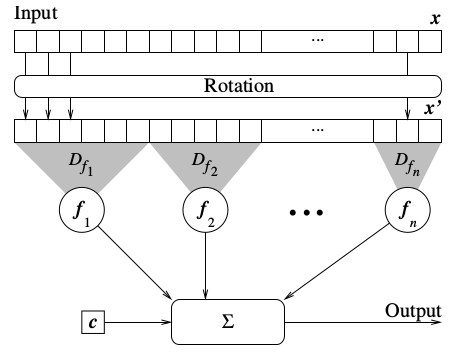
\includegraphics[scale=0.5]{images/composicion}
  				\caption{Composición de funciones.}
				\end{figure}

\newpage
 
%%%%%%%%%%%%%%%%%%%%%%%%%%%%%%%%%%%%%%%%%%%%%%%%%%%%%%%%%%%%%%%%%%%%%%%%%%%%%% 
\section{Estudio de la Parametrización y Rendimiento}\label{sec:PARAM}

En esta sección trataremos el estudio de los parámetros empleados por cada uno de los algoritmos y como afectan al desempeño de los mismos. \\

Un parámetro común a todos los algoritmos desarrollados es el tamaño de la población, y es por ello que, se emplearán los mismos tamaños de población, $popsize = 20, 50, 75, 100$, para estudiar el rendimiento de cada algoritmo, a excepción del algoritmo SA (Sección \ref{sec:SA}) que debido a que se trata de una meta-heurística de trayectoria se empleará únicamente un individuo.

\subsection{OBL-CPSO}\label{sec:paramOBL_CPSO}

En el diseño del algoritmo OBL-CPSO (Sección \ref{sec:OBL-CPSO}) sólo se contempla la utilización de un parámetro, el tamaño de población. Es por ello, que los experimentos realizados con este algoritmo buscan encontrar el tamaño de población más adecuado para su rendimiento. A continuación, podemos ver una comparativa de los experimentos realizados con $popsize = 20, 50, 75, 100$ en la que se presentan los valores de media ($\mu$), mediana ($\tilde{x}$) y desviación típica ($\sigma$) para las 18 funciones propuestas por el concurso GenOpt. \\
\begin{table}[!ht]
    \centering
    \resizebox{\textwidth}{!}{\begin{tabular}{LLLLLLLLLLLLLLLL}
    \toprule
      \multicolumn{3}{r}{OBL-CPSO-20} & \multicolumn{3}{r}{OBL-CPSO-50} & \multicolumn{3}{r}{OBL-CPSO-75} & \multicolumn{3}{r}{OBL-CPSO-100} \\
      & \mu & \tilde{x} & \sigma & \mu & \tilde{x} & \sigma & \mu & \tilde{x} & \sigma & \mu & \tilde{x} & \sigma\\
      \cmidrule(l){2-4} \cmidrule(l){5-7} \cmidrule(l){8-10} \cmidrule(l){11-13}
       \midrule
    f_{0} & 4.361e-01 & 2.041e-01 & 4.492e-01 & {\bf 3.937e-01} & {\bf 1.255e-01} & 4.193e-01 & 4.095e-01 & 1.364e-01 & 4.224e-01 & 1.228e+00 & 1.218e+00 & 2.404e-01 \\
f_{1} & 1.776e+00 & 1.681e+00 & 4.699e-01 & 1.464e+00 & 1.401e+00 & 2.359e-01 & {\bf 1.403e+00} & {\bf 1.351e+00} & 2.047e-01 & 3.706e+00 & 3.572e+00 & 7.136e-01 \\
f_{2} & {\bf 7.417e-01} & 1.002e+00 & 4.173e-01 & 7.657e-01 & {\bf 1.002e+00} & 3.618e-01 & 7.968e-01 & 1.004e+00 & 3.407e-01 & 1.250e+00 & 1.227e+00 & 1.530e-01 \\
f_{3} & 1.779e+00 & 1.699e+00 & 4.513e-01 & 1.455e+00 & 1.402e+00 & 2.441e-01 & {\bf 1.373e+00} & {\bf 1.350e+00} & 1.722e-01 & 3.708e+00 & 3.572e+00 & 7.161e-01 \\
f_{4} & 7.822e-01 & {\bf 1.003e+00} & 4.026e-01 & {\bf 7.764e-01} & 1.003e+00 & 3.803e-01 & 8.439e-01 & 1.004e+00 & 3.219e-01 & 1.248e+00 & 1.216e+00 & 1.645e-01 \\
f_{5} & 1.790e+00 & 1.698e+00 & 5.522e-01 & 1.451e+00 & 1.406e+00 & 2.479e-01 & {\bf 1.423e+00} & {\bf 1.357e+00} & 2.284e-01 & 3.707e+00 & 3.572e+00 & 7.162e-01 \\
f_{6} & 9.041e-01 & 3.609e-01 & 1.297e+00 & 5.852e-01 & 3.130e-01 & 7.651e-01 & {\bf 4.691e-01} & {\bf 2.570e-01} & 4.897e-01 & 3.368e+00 & 2.636e+00 & 2.445e+00 \\
f_{7} & 1.057e+01 & 1.014e+01 & 4.274e+00 & {\bf 8.992e+00} & 8.667e+00 & 3.394e+00 & 9.134e+00 & {\bf 8.482e+00} & 3.717e+00 & 2.545e+01 & 2.466e+01 & 6.987e+00 \\
f_{8} & 5.837e-01 & 3.580e-01 & 6.216e-01 & 3.908e-01 & {\bf 2.501e-01} & 4.752e-01 & {\bf 3.449e-01} & 2.537e-01 & 3.115e-01 & 2.202e+00 & 1.999e+00 & 1.283e+00 \\
f_{9} & 5.574e+00 & 5.209e+00 & 2.245e+00 & 4.881e+00 & 4.840e+00 & 1.817e+00 & {\bf 4.720e+00} & {\bf 4.588e+00} & 1.643e+00 & 1.276e+01 & 1.279e+01 & 3.019e+00 \\
f_{10} & 6.175e-03 & 4.830e-03 & 5.254e-03 & 4.564e-03 & 3.010e-03 & 3.711e-03 & {\bf 3.874e-03} & {\bf 2.688e-03} & 3.495e-03 & 1.661e-02 & 1.440e-02 & 1.151e-02 \\
f_{11} & 4.735e-02 & 4.723e-02 & 1.483e-02 & 4.155e-02 & 3.961e-02 & 1.488e-02 & {\bf 4.151e-02} & {\bf 3.904e-02} & 1.285e-02 & 8.903e-02 & 8.608e-02 & 2.672e-02 \\
f_{12} & 4.103e-02 & 2.806e-02 & 4.074e-02 & {\bf 2.463e-02} & {\bf 1.685e-02} & 2.296e-02 & 3.093e-02 & 2.092e-02 & 3.662e-02 & 4.394e-01 & 3.230e-01 & 3.904e-01 \\
f_{13} & 8.880e-02 & 8.295e-02 & 3.394e-02 & 8.708e-02 & 8.431e-02 & 2.912e-02 & {\bf 8.200e-02} & {\bf 8.032e-02} & 2.643e-02 & 2.611e-01 & 2.452e-01 & 1.296e-01 \\
f_{14} & 1.026e-01 & 3.233e-02 & 1.907e-01 & 3.723e-02 & 2.042e-02 & 4.753e-02 & {\bf 3.049e-02} & {\bf 1.543e-02} & 4.289e-02 & 1.381e+00 & 1.147e+00 & 1.006e+00 \\
f_{15} & 1.317e-01 & 1.180e-01 & 5.010e-02 & 1.198e-01 & 1.121e-01 & 3.953e-02 & {\bf 1.196e-01} & {\bf 1.115e-01} & 4.406e-02 & 4.437e-01 & 3.095e-01 & 4.113e-01 \\
f_{16} & 1.516e-02 & 1.252e-02 & 1.090e-02 & 1.380e-02 & 1.075e-02 & 1.142e-02 & {\bf 1.201e-02} & {\bf 1.052e-02} & 8.260e-03 & 4.439e-02 & 3.137e-02 & 4.109e-02 \\
f_{17} & 2.666e-01 & 2.286e-01 & 1.587e-01 & 2.049e-01 & 1.744e-01 & 1.091e-01 & {\bf 1.845e-01} & {\bf 1.687e-01} & 8.040e-02 & 3.330e+00 & 2.985e+00 & 1.709e+00 \\
    \bottomrule
    \end{tabular}}
    \captionsetup{justification=centering}
    \caption{Comparativa del algoritmo OBL-CPSO con diferentes tamaños de población.}    
\end{table}

Como podemos observar, en negrita se muestran los mejores valores obtenidos para cada una de las funciones a optimizar 

\newpage
\subsection{CMA-ES}\label{sec:paramCMA_ES}

El diseño del algoritmo CMA-ES, como detallamos en la sección \ref{sec:CMA}, sólo necesita la definición de dos parámetros iniciales para comenzar su ejecución, el tamaño de la población a emplear y el valor de sigma ($\sigma$) inicial. \\ Para evaluar el rendimiento del algoritmo variando estos dos parámetros, hemos realizado un total de 12 experimentos. \\

El tamaño de la población, como especificamos en el inicio de la sección, tomará los siguientes valores $popsize = 20, 50, 75, 100$. \\
En cuanto al parámetro $\sigma$, los valores que tomará serán $\sigma = 0.3; 0.8; 2.0$. La elección de estos valores se basa en que el parámetro $\sigma$ determina la variación incluida en cada nueva generación de la población y teniendo en cuenta esto, unos valores de $\sigma$ pequeños como 0.3 y 0.8 harán que el algoritmo se comporte como una búsqueda local, y al contrario, como una búsqueda global, con valores grandes de $\sigma$ como 2.0 \cite{CMA1}. \\

A continuación podemos observar una tabla en la muestran los resultados de la  evaluación el rendimiento de las mejores configuraciones obtenidas de las 12 configuraciones totales. Estas configuraciones son CMA\_ES-$2-50$, CMA\_ES-$0.3-50$ y CMA\_ES-$0.3-100$, mostrando para cada configuración los valores de media ($\mu$), mediana ($\tilde{x}$) y desviación típica ($\sigma$) para las 18 funciones propuestas por el concurso GenOpt. La nomenclatura utilizada es la siguiente: CMA\_ES-$\sigma-popsize$. \\
\begin{table}[!ht]
    \centering
    \resizebox{\textwidth}{!}{\begin{tabular}{LLLLLLLLLLLLLLLL}
    \toprule
      \multicolumn{3}{r}{CMA\_ES-$2-50$} & \multicolumn{3}{r}{CMA\_ES-$0.3-50$} & \multicolumn{3}{r}{CMA\_ES-$0.8-50$} \\
      & \mu & \tilde{x} & \sigma & \mu & \tilde{x} & \sigma & \mu & \tilde{x} & \sigma\\
      \cmidrule(l){2-4} \cmidrule(l){5-7} \cmidrule(l){8-10} 
       \midrule
    f_{0} & {\bf 8.503e-01} & {\bf 1.000e+00} & 2.677e-01 & 6.503e+00 & 1.089e+00 & 2.677e-01 & 8.503e-01 & 1.000e+00 & 2.677e-01 \\
f_{1} & {\bf 1.145e+00} & {\bf 1.121e+00} & 9.401e-02 & 1.145e+00 & 1.331e+00 & 9.401e-02 & 1.145e+00 & 1.121e+00 & 9.401e-02 \\
f_{2} & {\bf 9.650e-01} & {\bf 1.000e+00} & 1.102e-01 & 6.890e-01 & 1.120e+00 & 1.102e-01 & 9.650e-01 & 1.000e+00 & 1.102e-01 \\
f_{3} & {\bf 1.145e+00} & {\bf 1.127e+00} & 9.699e-02 & 1.175e+00 & 1.197e+00 & 9.699e-02 & 1.145e+00 & 1.127e+00 & 9.699e-02 \\
f_{4} & {\bf 9.568e-01} & {\bf 1.000e+00} & 1.375e-01 & 7.544e-01 & 1.000e+00 & 1.375e-01 & 9.568e-01 & 1.000e+00 & 1.375e-01 \\
f_{5} & {\bf 1.139e+00} & {\bf 1.107e+00} & 9.068e-02 & 2.177e+00 & 1.107e+00 & 9.068e-02 & 1.139e+00 & 1.107e+00 & 9.068e-02 \\
f_{6} & {\bf 7.098e-03} & {\bf 2.675e-03} & 1.102e-02 & 6.068e-03 & 2.895e-03 & 1.102e-02 & 7.098e-03 & 2.675e-03 & 1.102e-02 \\
f_{7} & {\bf 3.485e+00} & {\bf 3.206e+00} & 1.737e+00 & 4.785e+00 & 3.206e+00 & 1.737e+00 & 3.485e+00 & 3.206e+00 & 1.737e+00 \\
f_{8} & {\bf 1.114e-02} & {\bf 3.920e-03} & 2.502e-02 & 1.184e-02 & 3.500e-03 & 2.502e-02 & 1.114e-02 & 3.920e-03 & 2.502e-02 \\
f_{9} & {\bf 1.801e+00} & {\bf 1.713e+00} & 8.352e-01 & 2.881e+00 & 1.503e+00 & 8.352e-01 & 1.801e+00 & 1.713e+00 & 8.352e-01 \\
f_{10} & {\bf 2.323e-02} & {\bf 2.214e-02} & 2.532e-02 & 1.393e-02 & 2.124e-02 & 2.532e-02 & 2.323e-02 & 2.214e-02 & 2.532e-02 \\
f_{11} & {\bf 5.283e-02} & {\bf 5.061e-02} & 1.399e-02 & 3.883e-02 & 5.031e-02 & 1.399e-02 & 5.283e-02 & 5.061e-02 & 1.399e-02 \\
f_{12} & {\bf 2.242e-04} & {\bf 1.147e-04} & 5.236e-04 & 4.442e-04 & 1.147e-04 & 5.236e-04 & 2.242e-04 & 1.147e-04 & 5.236e-04 \\
f_{13} & {\bf 3.018e-02} & {\bf 2.998e-02} & 7.994e-03 & 2.018e-02 & 2.998e-02 & 7.994e-03 & 3.018e-02 & 2.998e-02 & 7.994e-03 \\
f_{14} & {\bf 1.443e-04} & {\bf 2.946e-05} & 3.504e-04 & 1.443e-04 & 2.946e-05 & 3.504e-04 & 1.443e-04 & 2.946e-05 & 3.504e-04 \\
f_{15} & {\bf 4.870e-02} & {\bf 4.838e-02} & 1.111e-02 & 4.870e-02 & 4.838e-02 & 1.111e-02 & 4.870e-02 & 4.838e-02 & 1.111e-02 \\
f_{16} & {\bf 9.820e-04} & {\bf 2.520e-04} & 5.633e-03 & 9.820e-04 & 2.520e-04 & 5.633e-03 & 9.820e-04 & 2.520e-04 & 5.633e-03 \\
f_{17} & {\bf 3.485e-02} & {\bf 3.375e-02} & 9.540e-03 & 3.485e-02 & 3.375e-02 & 9.540e-03 & 3.485e-02 & 3.375e-02 & 9.540e-03 \\
    \bottomrule
    \end{tabular}}
    \captionsetup{justification=centering}
    \caption{Comparativa de algunas de las instancias CMA\_ES-$\sigma-popsize$.}    
\end{table}

Como podemos observar, los resultados destacados en negrita muestran la mejor configuración, CMA\_ES-$2-50$, de las tres presentadas aunque, estos resultados son idénticos a los obtenidos con la configuración CMA\_ES-$0.8-50$. Esto es así debido a la estratégia de reinicio empleada en nuestro algoritmo, la cual define $\sigma = 2$ cuando es empleada.

\newpage

\subsection{HSAGS}\label{sec:paramSA}

Por último, el algoritmo HSAGS (sección \ref{sec:SA}) presenta únicamente un parámetro, la temperatura inicial. Según la literatura \cite{metabook}, inicialmente este parámetro debe tener un valor elevado, y es por ello, por lo que los valores con los que hemos evaluado el rendimiento de este algoritmo han sido $Temp_{0} = 500, 1000, 10000$. A continuación, podemos ver una comparativa del \textbf{valor de error} obtenido por cada experimento en cada una de las funciones propuestas por el concurso GenOpt. Como se puede observar, los valores resaltados en negrita muestran el valor de error mínimo alcanzado para cada una de las funciones propuestas por el concurso GenOpt y qué configuración del algoritmo HSAGS la obtuvo. Además, las flechas bidireccionales muestran que los valores de error obtenidos por las configuraciones apuntadas por dichas flechas son muy similares. La nomenclatura empleada es la siguiente: HSAGS-$TEMP_{0}$.

\begin{table}[!ht]
    \centering
    \fontsize{11}{9}\selectfont
    \begin{tabular}{LLLLLLL}
    \toprule
    & \textbf{HSAGS-500} &  & \textbf{HSAGS-1000} & & \textbf{HSAGS-10000} \\
      \midrule
    f_{0} & 8.060e-01 & \leftrightarrow & \textbf{9.338e-01} & \leftrightarrow & 7.384e-01 \\
f_{1} & {\bf 0.000e+00} &  & 9.732e-01 & \leftrightarrow & 9.732e-01 \\
f_{2} & 9.241e-01 & \leftrightarrow & 9.270e-01 & \leftrightarrow & \textbf{9.711e-01} \\
f_{3} & {\bf 0.000e+00} &  & {\bf 0.000e+00} &  & {\bf 0.000e+00} &  \\
f_{4} & 7.369e-01 & \leftrightarrow & \textbf{8.174e-01} & \leftrightarrow & 5.917e-01 \\ 
f_{5} & 9.481e-01 & \leftrightarrow & 9.460e-01 & \leftrightarrow & \textbf{9.978e-01} \\
f_{6} & 9.961e-01 & \leftrightarrow & 9.971e-01 & \leftrightarrow & \textbf{9.990e-01} \\
f_{7} & \textbf{9.990e-01} & \leftrightarrow & 9.971e-01 & \leftrightarrow & 9.981e-01 \\
f_{8} & {\bf 0.000e+00} &  & 1.000e+00 & \leftrightarrow & 1.000e+00 \\
f_{9} & 1.000e+00 & \leftrightarrow & 1.000e+00 & \leftrightarrow & {\bf 0.000e+00} &  \\
f_{10} & \textbf{9.990e-01} & \leftrightarrow & 9.971e-01 & \leftrightarrow & 9.981e-01 \\ 
f_{11} & 9.942e-01 & \leftrightarrow & 9.961e-01 & \leftrightarrow & \textbf{9.990e-01} \\
f_{12} & \textbf{1.000e+00} & \leftrightarrow & 1.000e+00 & \leftrightarrow & 1.000e+00 \\
f_{13} & \textbf{9.990e-01} & \leftrightarrow & 9.990e-01 & \leftrightarrow & 1.000e+00 \\
f_{14} & \textbf{1.000e+00} & \leftrightarrow & 1.000e+00 & \leftrightarrow & 1.000e+00 \\
f_{15} & \textbf{1.000e+00} & \leftrightarrow & 1.000e+00 & \leftrightarrow & 1.000e+00 \\
f_{16} & 1.000e+00 & \leftrightarrow & \textbf{9.990e-01} & \leftrightarrow & 9.990e-01 \\
f_{17} & \textbf{1.000e+00} & \leftrightarrow & 1.000e+00 & \leftrightarrow & 1.000e+00 \\
    \bottomrule
    \end{tabular}
     \captionsetup{justification=centering}
    \caption{Comparativa del algoritmo HSAGS con diferentes valores de temperatura inicial.}    
\end{table}

\newpage

\subsection{Comparativa de Rendimiento entre Algoritmos}\label{sec:compALL}

En la siguiente tabla, se presenta una comparativa de los valores media ($\mu$), mediana ($\tilde{x}$) y desviación típica ($\sigma$) de las mejores configuraciones conseguidas con cada uno de los algoritmos implementados. Como podemos apreciar, el algoritmo CMA-ES \cite{CMA} (Sección \ref{sec:CMA}) consigue los mejores resultados para las 18 funciones propuestas por el concurso GenOpt. Debido a estos resultados, el algoritmo CMA-ES fue escogido para competir en la fase final del concurso.

\begin{table}[!ht]
    \centering
    \resizebox{\textwidth}{!}{\begin{tabular}{LLLLLLLLLL}
    \toprule
     \multicolumn{3}{r}{CMA\_ES-$2-50$} & \multicolumn{3}{r}{OBL-CPSO-75} & \multicolumn{3}{r}{HSAGS-500} \\
     & \mu & \tilde{x} & \sigma & \mu & \tilde{x} & \sigma & \mu & \tilde{x} & \sigma\\
     \cmidrule(l){2-4} \cmidrule(l){5-7} \cmidrule(l){8-10}
       \midrule
    f_{0} & 8.503e-01 & 1.000e+00 & 2.677e-01 & {\bf4.095e-01} & {\bf1.364e-01} & 4.224e-01 & 3.875e+00 & 3.731e+00 & 8.967e-01\\
f_{1} & {\bf 1.145e+00} & {\bf 1.121e+00} & 9.401e-02 & 1.403e+00 & 1.351e+00 & 2.047e-01 & 1.065e+01 & 1.052e+01 & 1.439e+00\\
f_{2} & {\bf 9.650e-01} & {\bf 1.000e+00} & 1.102e-01 & 7.968e-01 & 1.004e+00 & 3.407e-01 & 3.878e+00 & 3.731e+00 & 8.982e-01\\
f_{3} & {\bf 1.145e+00} & {\bf 1.127e+00} & 9.699e-02 & 1.373e+00 & 1.350e+00 & 1.722e-01 & 1.065e+01 & 1.052e+01 & 1.439e+00\\
f_{4} & {\bf 9.568e-01} & {\bf 1.000e+00} & 1.375e-01 & 8.439e-01 & 1.004e+00 & 3.219e-01 & 9.568e-01 & 1.000e+00 & 1.375e-01 \\
f_{5} & {\bf 1.139e+00} & {\bf 1.107e+00} & 9.068e-02 & 1.423e+00 & 1.357e+00 & 2.284e-01 & 1.064e+01 & 1.050e+01 & 1.435e+00\\
f_{6} & {\bf 7.098e-03} & {\bf 2.675e-03} & 1.102e-02 & 4.691e-01 & 2.570e-01 & 4.897e-01 & 1.373e+01 & 1.227e+01 & 6.326e+00\\
f_{7} & {\bf 3.485e+00} & {\bf 3.206e+00} & 1.737e+00 & 9.134e+00 & 8.482e+00 & 3.717e+00 & 4.560e+01 & 4.423e+01 & 1.053e+01\\
f_{8} & {\bf 1.114e-02} & {\bf 3.920e-03} & 2.502e-02 & 3.449e-01 & 2.537e-01 & 3.115e-01 & 6.038e+00 & 6.183e+00 & 1.809e+00\\
f_{9} & {\bf 1.801e+00} & {\bf 1.713e+00} & 8.352e-01 & 4.720e+00 & 4.588e+00 & 1.643e+00 & 1.903e+01 & 1.891e+01 & 3.118e+00\\
f_{10} & {\bf 2.323e-02} & {\bf 2.214e-02} & 2.532e-02 & 3.874e-03 &  2.688e-03 & 3.495e-03 & 1.270e-01 &   5.255e-02  & 2.558e-01\\
f_{11} & {\bf 5.283e-02} & {\bf 5.061e-02} & 1.399e-02 & 4.151e-02 &  3.904e-02 & 1.285e-02 & 4.264e+00 &   1.808e-01  & 2.459e+01\\
f_{12} & {\bf 2.242e-04} & {\bf 1.147e-04} & 5.236e-04 & 3.093e-02 & 2.092e-02 & 3.662e-02 & 5.330e+00 &   5.016e+00  & 2.499e+00\\
f_{13} & {\bf 3.018e-02} & {\bf 2.998e-02} & 7.994e-03 & 8.200e-02 & 8.032e-02 & 2.643e-02 & 2.689e+00 &   2.567e+00  & 1.265e+00\\
f_{14} & {\bf 1.443e-04} & {\bf 2.946e-05} & 3.504e-04 & 3.049e-02 &  1.543e-02 & 4.289e-02 & 8.964e+00 &   8.338e+00  & 4.235e+00\\
f_{15} & {\bf 4.870e-02} & {\bf 4.838e-02} & 1.111e-02 & 1.196e-01 &  1.115e-01 & 4.406e-02 & 1.009e+01 &   8.802e+00  & 5.327e+00\\\
f_{16} & {\bf 9.820e-04} & {\bf 2.520e-04} & 5.633e-03 & 1.201e-02 &  1.052e-02 & 8.260e-03  & 4.049e+00 &   3.340e+00  & 3.172e+00\\
f_{17} & {\bf 3.485e-02} & {\bf 3.375e-02} & 9.540e-03 & 1.845e-01 &  1.687e-01 & 8.040e-02 & 1.603e+01 &   1.465e+01  & 5.702e+00\\
    \bottomrule
    \end{tabular}}
    \captionsetup{justification=centering}
    \caption{Comparativa de las mejores configuraciones de cada algoritmo implementado.}    
\end{table}
\newpage

%%%%%%%%%%%%%%%%%%%%%%%%%%%%%%%%%%%%%%%%%%%%%%%%%%%%%%%%%%%%%%%%%%%%%%%%%%%%%%
\section{Clasificación en el Concurso GenOpt}\label{sec:Competition}

Desde la organización del concurso GenOpt proponen varios criterios para clasificar los algoritmos enviados por los participantes. Estos criterios pueden ser:

\begin{itemize}
    	  	\item \textbf{High Jump}: Mejor valor obtenido en los puntos de control.
    	  	\item \textbf{Target Shooting}: Éxito a la hora de alcanzar el óptimo global de la función.
    	  	\item \textbf{Biathlon Score}: Media entre el High Jump y Target Shooting.
\end{itemize}
Para obtener más detalles sobre como se calculan estas métricas, se recomienda la lectura del Manifesto del GenOpt\footnote{Dirección desde la que se puede obtener el Manifesto del concurso GenOpt: http://www.genopt.org/genopt.pdf.}.

A la vista de los resultados obtenidos en las diversas pruebas llevadas a cabo en el análisis de rendimiento \ref{sec:compALL}, decidimos emplear el algoritmo CMA-ES (Sección \ref{sec:CMA}) para participar en la fase final del concurso. \\
Con este algoritmo, el cual denominamos \textit{Hybrid Continuous Optimiser based on CMA-ES and a Global Neighbourhood Path Search (HCO-CMA-G)}, conseguimos la \textbf{tercera posición} en el ranking final según el parámetro \textbf{High Jump}, como podemos ver en la siguiente figura: 

\begin{figure}[!ht]
  \centering
	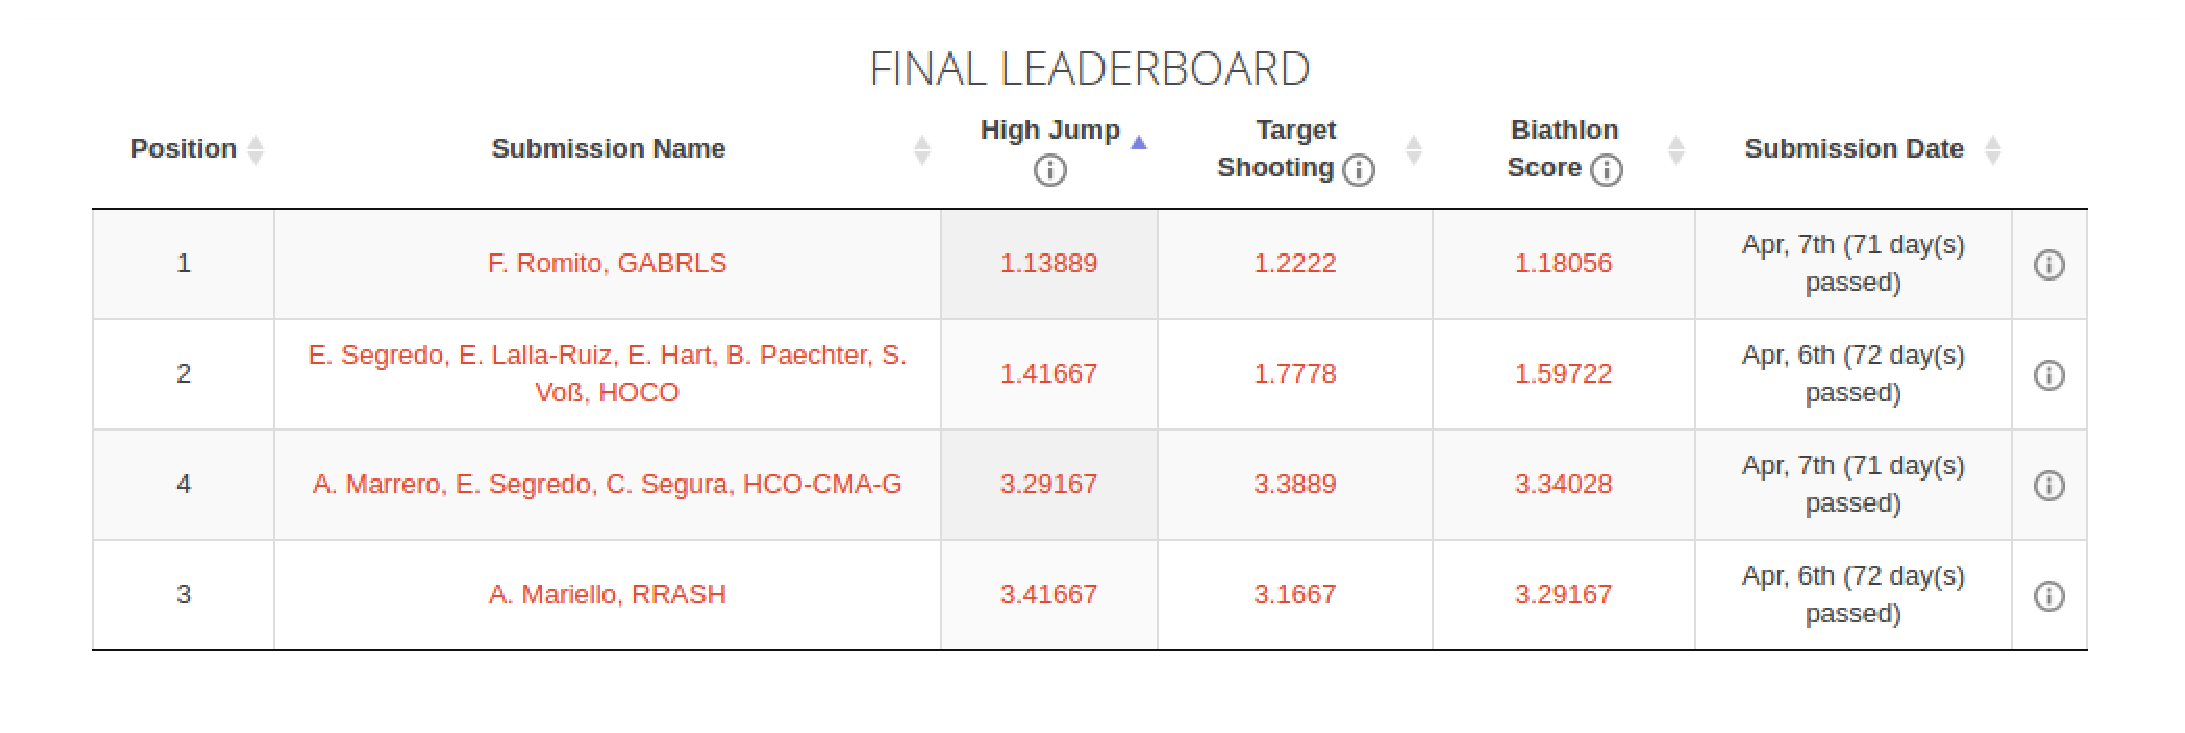
\includegraphics[scale=0.5]{images/final}
  \caption{Clasificación en el concurso GenOpt según High Jump.}
\end{figure}

\newpage

A continuación, podemos observar una comparativa del rendimiento entre los finalistas del concurso GenOpt basado en el criterio High Jump.

\begin{figure}[!ht]
  \centering
  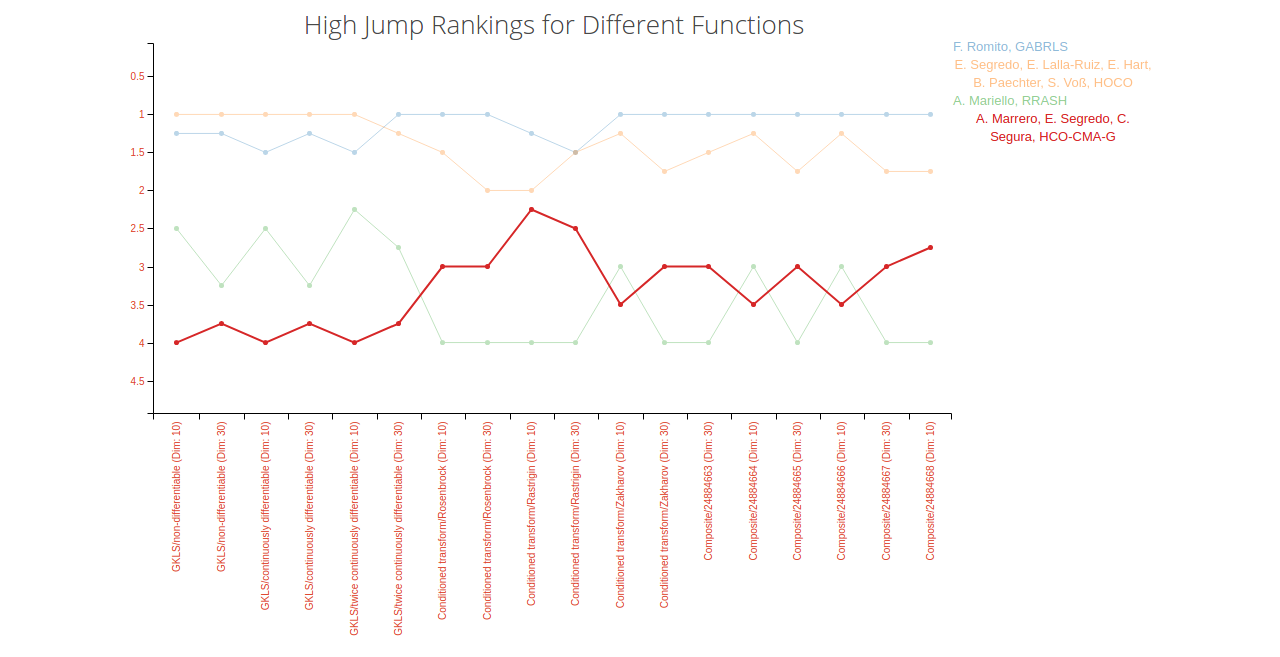
\includegraphics[scale=0.4]{images/highjump}
  \caption{Clasificación en el concurso GenOpt según High Jump.}
\end{figure}



%%%%%%%%%%%%%%%%%%%%%%%%%%%%%%%%%%%%%%%%%%%%%%%%%%%%%%%%%%%%%%%%%%%%%%%%%%%%%%%
\newpage{\pagestyle{empty}}
\thispagestyle{empty}

\chapter{Conclusiones y líneas futuras}
\label{chapter:Conclusiones}

%%%%%%%%%%%%%%%%%%%%%%%%%%%%%%%%%%%%%%%%%%%%%%%%%%%%%%%%%%%%%%%%%%%%%%%%%%%%%
% Chapter 5: Conclusiones y Trabajos Futuros 
%%%%%%%%%%%%%%%%%%%%%%%%%%%%%%%%%%%%%%%%%%%%%%%%%%%%%%%%%%%%%%%%%%%%%%%%%%%%%%%

%%%%%%%%%%%%%%%%%%%%%%%%%%%%%%%%%%%%%%%%%%%%%%%%%%%%%%%%%%%%%%%%%%%%%%%%%%%%%%%
\section{Conclusiones}

Durante la elaboración de este Trabajo de Fin de Grado hemos obtenido varias conclusiones que destacaremos a continuación.

En primer lugar, trabajar con algoritmos que requieren una gran cantidad de parámetros, como es el caso del algoritmo CMA-ES u OBL-CPSO, hace que la evaluación del rendimiento del algoritmo sea más compleja dado que por cada parámetro se incrementa significativamente la cantidad de experimentos a realizar para probar el rendimiento del mismo. Aún así, en el caso del algoritmo CMA-ES, la naturaleza auto-reguladora del algoritmo facilita en cierta medida esta tarea. 

Hemos de destacar además que, debido al gran número de funciones propuestas por el concurso GenOpt, las modificaciones realizadas a los algoritmos resultaron difíciles de evaluar dado que en bastantes ocasiones, la mejora era simplemente en funciones concretas y en conjunto, los resultados no variaban significativamente para considerar dicha modificación.\\

Merece la pena mencionar que el algoritmo CMA-ES (Sección \ref{sec:CMA}) consiguió el \textbf{tercer mejor puesto} según el criterio \textbf{High Jump} en la clasificación final del concurso GenOpt.

Finalmente, y considerando los resultados obtenidos por las técnicas implementadas, podemos concluir que el algoritmo CMA-ES es el más eficaz resolviendo el conjunto de problemas propuesto por GenOpt.


%%%%%%%%%%%%%%%%%%%%%%%%%%%%%%%%%%%%%%%%%%%%%%%%%%%%%%%%%%%%%%%%%%%%%%%%%%%%%%%
\section{Líneas de Trabajo Futuras}

El trabajo desarrollado en este proyecto puede servir como base para comprobar el rendimiento de diferentes técnicas meta-heurísticas a la hora de resolver problemas de optimización continua. \\
Además, como líneas de trabajo futuras se prevé la mejora algunas de las técnicas implementadas, así como un estudio más intensivo de los parámetros, con vistas a participar en la siguiente edición del concurso GenOpt.

%%%%%%%%%%%%%%%%%%%%%%%%%%%%%%%%%%%%%%%%%%%%%%%%%%%%%%%%%%%%%%%%%%%%%%%%%%%%%%%
\newpage{\pagestyle{empty}}
\thispagestyle{empty}

\chapter{Summary and Conclusions }
\label{chapter:ingles}

%%%%%%%%%%%%%%%%%%%%%%%%%%%%%%%%%%%%%%%%%%%%%%%%%%%%%%%%%%%%%%%%%%%%%%%%%%%%%
% Chapter 6: Summary and Conlusions
%%%%%%%%%%%%%%%%%%%%%%%%%%%%%%%%%%%%%%%%%%%%%%%%%%%%%%%%%%%%%%%%%%%%%%%%%%%%%%%

%++++++++++++++++++++++++++++++++++++++++++++++++++++++++++++++++++++++++++++++
\section{Conclusions}

Through the development of this degree thesis we have reached the following conclusions: 

First of all, the fact of working with algorithms which use a high amount of parameters, like CMA-ES or OBL-CPSO, increases the complexity to evaluate the performance of the algorithms due to the fact that the number of possible tests increases with each parameter. Even though, the self-regulation nature of the algorithms like CMA-ES facilitates this task.

Furthermore, as a result of the large amount of proposed functions by the GenOpt contest, the task of assessing a new modification was really difficult. In many times, results were only improved for a low number of the proposed functions. \\

It is worth to be mentioned that the CMA-ES algorithm (Section \ref{sec:CMA}) accomplished the \textbf{third place} in the final leaderboard of the GenOpt contest considering the High Jump criterion.

Finally, taking into account the obtained results by the developed algorithms, we can conclude that the algorithm CMA-ES was the most effective approach solving the functions proposed by the GenOpt contest.



%%%%%%%%%%%%%%%%%%%%%%%%%%%%%%%%%%%%%%%%%%%%%%%%%%%%%%%%%%%%%%%%%%%%%%%%%%%%%%%
\section{Future work}

The work developed in this project could be a starting point to test the performance of different meta-heuristic algorithms for solving continuos optimization problems.\\

A potential line of future work may be the improvement of the different tested algorithms, with the aim of participating in future editions of the GenOpt contest.


%%%%%%%%%%%%%%%%%%%%%%%%%%%%%%%%%%%%%%%%%%%%%%%%%%%%%%%%%%%%%%%%%%%%%%%%%%%%%%%
\newpage{\pagestyle{empty}}
\thispagestyle{empty}

\chapter{Presupuesto}
\label{chapter:Presupuesto}

%%%%%%%%%%%%%%%%%%%%%%%%%%%%%%%%%%%%%%%%%%%%%%%%%%%%%%%%%%%%%%%%%%%%%%%%%%%%%
% Chapter 7: Presupuesto
%%%%%%%%%%%%%%%%%%%%%%%%%%%%%%%%%%%%%%%%%%%%%%%%%%%%%%%%%%%%%%%%%%%%%%%%%%%%%%%

%++++++++++++++++++++++++++++++++++++++++++++++++++++++++++++++++++++++++++++++

En este capítulo se va a detallar el presupuesto para la realización de este Trabajo de Fin de Grado.

\subsection{Ingeniero Informático}

En la siguiente tabla se detallan todas las actividades llevadas a cabo durante el presente Trabajo de Fin de Grado indicando la duración en horas de cada una de ellas y el coste en Euros. 
Se ha establecido un precio base de 20 Euros para cada hora de trabajo. El coste total del desarrollo de la investigación es de 5300 Euros.
\begin{table}[h]
    \begin{tabular}{|c|c|c|}
    \hline
    Actividad                                                & Duración(horas) & Coste    \\ \hline
    Investigación de las técnicas algorítmicas existentes    & 20              & 400      \\ \hline
    Selección de los algoritmos a desarrollar                & 15               & 300      \\ \hline
    Desarrollo del algoritmo OBL-CPSO                        & 40              & 800      \\ \hline
    Estudio de los parámetros del algoritmo OBL-CPSO         & 20              & 400      \\ \hline
    Desarrollo del algoritmo CMA-ES                          & 55              & 1100     \\ \hline
    Estudio de los parámetros del algoritmo CMA-ES           & 20              & 400      \\ \hline
    Desarrollo del algoritmo Simulated Annealing             & 20              & 400      \\ \hline
    Estudio de los parámetros de Simualted Annealing         & 40              & 800      \\ \hline
    Desarrollo de las métricas propuestas por GENOPT         & 20              & 400      \\ \hline
    Obtención de las gráficas con los resultados del estudio & 20              & 400      \\ \hline
    Redacción de la memoria                                  & 30              & 600      \\ \hline
    \end{tabular}
    \caption {Actividades}
\end{table}

\begin{table}[h]
    \centering
    \begin{tabular}{|c|c|}
    \hline
    Coste total & 11510 Euros \\ \hline
    \end{tabular}
    \caption {Coste total de las actividades}
\end{table}
\\
\bigskip    
\\

\subsection{Materiales}
Por otra parte, también se ha usado el siguiente equipamiento durante el desarrollo de este Trabajo de Fin de Grado

\begin{table}[h]
    \centering
    \begin{tabular}{|c|c|}
    \hline
    Equipo                 & Coste(Euros) \\ \hline
    Acer Aspire V3-772g    & 800          \\ \hline
    Monitor LG             & 120          \\ \hline
    Escritorio Skarsta     & 219          \\ \hline
    Silla de oficina Jules & 50           \\ \hline
    \end{tabular}
    \caption {Equipamiento}
\end{table}
\begin{table}[h]
    \centering
    \begin{tabular}{|c|c|}
    \hline
    Coste total & 1189 Euros \\ \hline
    \end{tabular}
    \caption {Coste del equipamiento}
\end{table}

\subsection{Coste Total}
Finalmente, el coste total del Trabajo de Fin de Grado sumando el coste de las actividades llevadas a cabo y el equipamiento utilizado para dicha labor es de 7189 Euros.

%%%%%%%%%%%%%%%%%%%%%%%%%%%%%%%%%%%%%%%%%%%%%%%%%%%%%%%%%%%%%%%%%%%%%%%%%%%%%%%

\addcontentsline{toc}{chapter}{Bibliografía}
\bibliographystyle{plain}

\bibliography{memtfg}
%\nocite{*}

%%%%%%%%%%%%%%%%%%%%%%%%%%%%%%%%%%%%%%%%%%%%%%%%%%%%%%%%%%%%%%%%%%%%%%%%%%%%%%%

\end{document}

